\begin{frame}{Step 1: Research and Analysis}
  \begin{itemize}
    \item \textbf{Exploring GEM5 Internals:} 
      \begin{itemize}
        \item Investigated the core components of GEM5 including CPU models, memory systems, and simulation flow.
        \item Found limited developer documentation — referred to the official \href{https://doxygen.gem5.org/develop/index.html}{Doxygen documentation \faLink}.
        \item Studied through 3,358 source files comprising 965,657 lines of code.
      \end{itemize}

    \item \textbf{Studying AVR Architecture:}
      \begin{itemize}
        \item Reviewed instruction set, register architecture, and interrupt handling for AVR microcontrollers.
      \end{itemize}

    \item \textbf{Feasibility Analysis:}
      \begin{itemize}
        \item Evaluated how a lightweight 16-bit AVR ISA could be integrated into GEM5’s CPU model framework.
        \item Focused on maintaining modularity and clean abstraction layers.
      \end{itemize}

    \item \textbf{Initial Outcomes:}
      \begin{itemize}
        \item Conducted a simulation-based evaluation titled \href{https://drive.google.com/file/d/13ZroHuWGLApYXLkeWA3SBIlMh6KzfCqq/view?usp=sharing}{\texttt{Comparative Study on Execution Speed \& CMR of Various ISAs \faLink.}} 
      \end{itemize}
  \end{itemize}
\end{frame}


\begin{frame}{Step 2: ISA Integration}
  \centering
  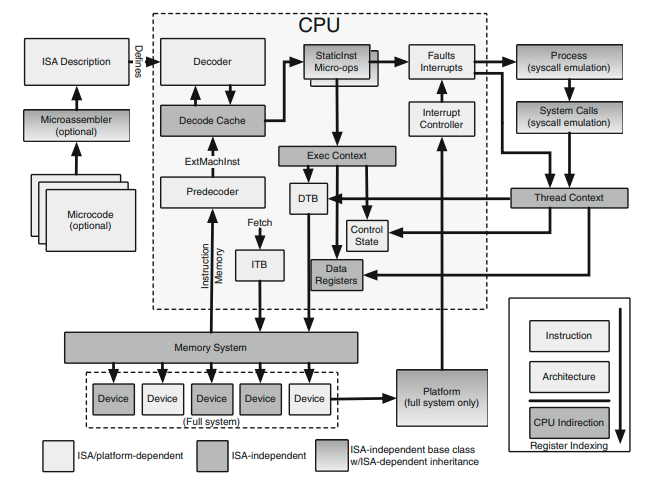
\includegraphics[width=0.55\textwidth]{images/impl.png}\\
  \textbf{Figure 3: }Dependence of gem5 components on ISA
\end{frame}

\begin{frame}{Step 2: ISA Integration}
  \begin{itemize}
    \item For the project we need to implement:
    \begin{itemize}
      \item ISA Description
      \item Decoder
      \item Fault Interrupts
      \item Predecoder
      \item Python Bindings to CPU \& I/O models.
      \item GUI for the simulator
    \end{itemize}
    \item For the begging a set of basic instructions are being implemented:
    \begin{itemize}
      \item \textbf{Arithmetic Instructions:} ADD, SUB
    \end{itemize}
    \item Current implementation includes:
    \begin{itemize}
      \item ISA Description with two above-mentioned instructions
      \item \texttt{AVRFault} for fault handling
      \item \textbf{Registers:} 32 general-purpose registers (R0-R31), SREG (Status Register)
      \item \textbf{Program Counter (PC):} 16-bit PC for instruction addressing
      \item \textbf{Instruction Fetch and Decode:} Basic fetch-decode-execute cycle
    \end{itemize}
  \end{itemize}
\end{frame}

\begin{frame}[fragile]{Step 2: ISA Integration}
  \begin{figure}
    \centering
      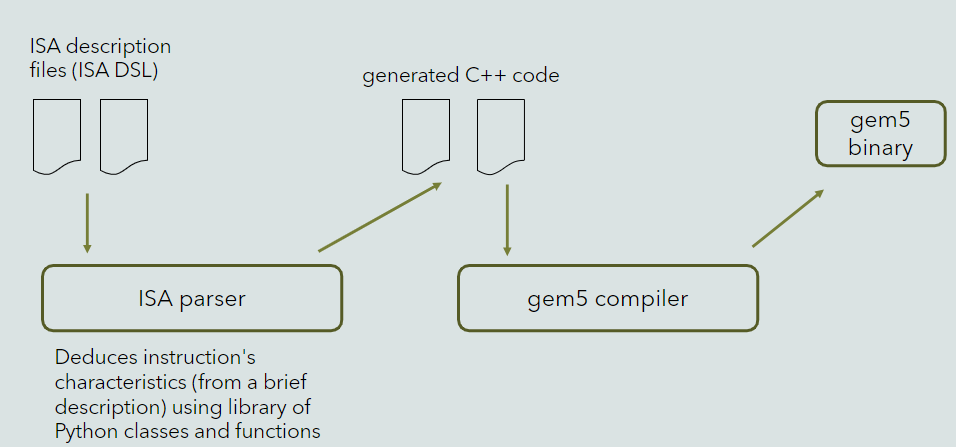
\includegraphics[width=0.8\textwidth]{images/flow.png}\\
      \textbf{Figure 4:} ISA description flow
  \end{figure}
\end{frame}

\begin{frame}[fragile]{Step 2: ISA Integration}
    Traversing the pipeline with `\texttt{add}' instruction:
    \begin{itemize}
      \item Bitfield definition for the instructions to be later used in the decoder: 
      \begin{lstlisting}[language=C++]
        def bitfield OPCODE    <15:10>;
        def bitfield REG_D     <8:4>;
        def bitfield REG_R     <3:0>;
        def bitfield IMM8      <7:0>;
      \end{lstlisting}
    \end{itemize}
\end{frame}

\begin{frame}[fragile]{Step 2: ISA Integration}
  \begin{itemize}
    \item Format declaration for \texttt{add} instruction. The declaration defines the output blocks for the code to be generated:
    \begin{lstlisting}[language=C++]
      def format Add(code, *opt_args) {{
        iop = InstObjParams(name, Name, 'AddOp',
                          {'code': code,
                            'predicate_test': predicateTest,
                            'op_class': 'gem5::enums::IntAlu'
                          },
                          opt_args)
        header_output = AddDeclare.subst(iop)
        decoder_output = AddConstructor.subst(iop)
        decode_block = AddDecode.subst(iop)
        exec_output = AddExecute.subst(iop)
        disasm_output = AddDisassembly.subst(iop)
    }};
    \end{lstlisting}
  \end{itemize}
\end{frame}

\begin{frame}[fragile]{Step 2: ISA Integration}
  \begin{itemize}
    \item Add class declaration including the constructor, execute method, disassembly method and PC advancement method:
    \begin{lstlisting}[language=C++]
      def template AddDeclare {{
        class %(class_name)s : public gem5::AVRISAInst::AVRStaticInst
        {
          public:
            %(class_name)s(gem5::AVRISAInst::MachInst machInst);
            Fault execute(ExecContext *, trace::InstRecord *) const override;
            std::string generateDisassembly(Addr pc,
                const loader::SymbolTable *symtab) const override;
            void advancePC(PCStateBase &pc_state) const;
        };
      }};
    \end{lstlisting}
  \end{itemize}
\end{frame}

\begin{frame}[fragile]{Step 2: ISA Integration}
  \begin{itemize}
    \item Generated C++ code for the Add class from the DSL code above:
    \begin{lstlisting}[language=C++]
      #undef OPCODE
      #define OPCODE	bits(machInst, 15, 10)
      #undef REG_D
      #define REG_D	bits(machInst,  8,  4)
      #undef REG_R
      #define REG_R	bits(machInst,  3,  0)
      #undef IMM8
      #define IMM8	bits(machInst,  7,  0)
      class Add : public gem5::AVRISAInst::AVRStaticInst
      {
        public:
          Add(gem5::AVRISAInst::MachInst machInst);
          Fault execute(ExecContext *, trace::InstRecord *) const override;
          std::string generateDisassembly(Addr pc,
              const loader::SymbolTable *symtab) const override;
          void advancePC(PCStateBase &pc_state) const;
      };
    \end{lstlisting}
  \end{itemize}
\end{frame}


\begin{frame}{Step 2: ISA Integration}
  \begin{itemize}
    \item Getting integration success with these two instructions opened door for further extending the instruction set.
    \item The groundwork for extension is laid out with the fault handling, PC management and register modeling. 
  \end{itemize}
\end{frame}